%%
% La siguiente plantilla esta basada en el siguiente enlace:
% http://academic.reed.edu/physics/courses/Physics332.s08/reports.html
% La plantilla original puede descargarse de ese sitio
% Se dejo parte del texto original en inglés para ilustar el uso de la plantilla
% Se hicieron algunas modificaciones para ajustar el idioma y otros detalles para 
% completar un reporte técnico breve pero muy puntual
% Modificación Inicial: Marco Aurelio Nuno Maganda - 11/SEP/2014
% 
% Enlace a la documentación del tipo de documento base (revtex4)
% http://mirror.hmc.edu/ctan/macros/latex/contrib/revtex/doc/latex/revtex/source/revtex4-1.pdf
%
% En algunas distribuciones es necesario instalar el paquete texlive-publishers
%
%\documentclass[letterpaper,aps,twocolumn,pre,nofootinbib]{revtex4}
%\documentclass[twocolumn]{article}
\documentclass[conference]{IEEEtran}

\usepackage[spanish]{babel}
\usepackage{amsmath,amssymb,amsfonts,amsthm}
\usepackage{graphicx}
%\usepackage{bbm}
\usepackage[utf8]{inputenc} % Caracteres en Español (Acentos, ñs)
\usepackage{url} % ACENTOS
\usepackage{hyperref} % Referencias
\usepackage{subfig}
\usepackage{lipsum}
\usepackage{balance}
\usepackage{algorithm}
\usepackage{algorithmic}


%%%%%%%%%%%%%%%%%%%%%%%%%%%%%%%%%%%%%%%%%%%%%
% PARCHE PARA ELIMINAR LA FECHA DEL DOCUMENTO
% 
\usepackage{etoolbox}
\makeatletter
% \frontmatter@RRAP@format is responsible for the parentheses
\patchcmd{\frontmatter@RRAP@format}{(}{}{}{}
\patchcmd{\frontmatter@RRAP@format}{)}{}{}{}
%\renewcommand\Dated@name{}
\makeatother	
% FIN DEL PARCHE
% 
%%%%%%%%%%%%%%%%%%%%%%%%%%%%%%%%%%%%%%%%%%%%%

%%%%%%%%%%%%%%%%%%%%%%%%%%%%%%%%%%%%%%%%%%%%%
% PARCHE PARA PERMIRIR UTILIZAR BIBLATEX EN ESTA PANTLLA
%\PassOptionsToPackage{square,numbers}{natbib}
%\RequirePackage{natbib}  
%%%%%%%%%%%%%%%%%%%%%%%%%%%%%%%%%%%%%%%%%%%%%

\usepackage[backend=bibtex,sorting=none]{biblatex}
% Estas lineas permiten romper los hipervinculos muy largos !!!!
\setcounter{biburllcpenalty}{7000}
\setcounter{biburlucpenalty}{8000}
\addbibresource{references.bib}

% Actualiza en automático la fecha de las citas de internet a la fecha de la compilación del documento
\usepackage{datetime}
\newdateformat{specialdate}{\twodigit{\THEDAY}-\twodigit{\THEMONTH}-\THEYEAR}
\date{\specialdate\today}

% la sentencia \burl en las citas... 
\usepackage[hyphenbreaks]{breakurl}

\renewcommand\spanishtablename{Tabla}
\renewcommand\spanishfigurename{Figura}

%\usepackage{datetime}
%\newdateformat{specialdate}{\twodigit{\THEDAY}-\twodigit{\THEMONTH}-\THEYEAR}
%\newdateformat{specialdate}{\twodigit{\THEDAY}-\THEYEAR}
%\date{\specialdate\today}


\begin{document}
%%%%%%%%%%%%%%%%%%%%%%%%%%%%%%%%%%%%%%%%%%%%%
% Definitions
%
%
% Define your special symbols here
%
%%%%%%%%%%%%%%%%%%%%%%%%%%%%%%%%%%%%%%%%%%%%%

% use to set width of figures
\newcommand{\breite}{0.9} %  for twocolumn
\newcommand{\RelacionFiguradoscolumnas}{0.9}
\newcommand{\RelacionFiguradoscolumnasPuntoCinco}{0.45}


%%%%%%%%%%%%%%%%%%%%%%%%%%%%%%%%%%%%%%%%%%%%%
% End Definitions
%%%%%%%%%%%%%%%%%%%%%%%%%%%%%%%%%%%%%%%%%%%%%


%Title of paper
\title{Reporte de Laboratorio X \\ Implementación de una aplicación móvil para detección de distraídos}

% Trabajo Individual
\author{\IEEEauthorblockN{
    Coyoy López Mario\IEEEauthorrefmark{1}\\
    Ledezma Donjuan Daniel Armando \IEEEauthorrefmark{1}\\
    Olivares Rodríguez Brayan \IEEEauthorrefmark{1}\\
    Torres Colorado Juan Daniel\IEEEauthorrefmark{1}
}
\IEEEauthorblockA{\IEEEauthorrefmark{1}Ingeniería en Tecnologías de la Información\\
Universidad Politécnica de Victoria}
}


%\date{}

\maketitle

\begin{abstract} 
\textbf{} En este proyecto se desarrolló un programa en C++ utilizando la biblioteca Qt para resolver el problema del cierre convexo (convex hull) utilizando varios algoritmos: Andrew's Monotone Chain, Graham Scan y Shamos. El programa permite al usuario crear un conjunto de puntos, editar estos puntos y luego aplicar los algoritmos mencionados para encontrar el cierre convexo del conjunto de puntos dado. La interfaz proporciona opciones intuitivas para ingresar y manipular los puntos, así como para seleccionar el algoritmo deseado. Se utilizan estructuras de datos como vectores y contenedores para almacenar y manipular los puntos, garantizando una ejecución eficiente de los algoritmos. El programa ofrece una experiencia interactiva y amigable para el usuario, facilitando la comprensión y la interacción con el proceso de cálculo del cierre convexo.
\end{abstract}


%\maketitle must follow title, authors, abstract, \pacs, and \keywords

\section{Introducción}

En el presente documento del proyecto de nombre ''Algoritmo Convex Hull'' se detalla el trabajo realizado y asignado como proyecto en equipo de la asignatura de Lenguajes y Autómatas en el lenguaje de programación C++ \cite{cpp}. El propósito de este proyecto tiene como motivo principal comprender los algoritmos de una envolvente convexa de manera visual, la cuál, cuente con una interfaz interactiva\cite{ui}.

La \textit{Convex Hull} (Envolvente Convexa) \cite{convex_hull-art} de un conjunto de puntos en un espacio euclidiano \cite{euclidiano} es el polígono convexo \cite{poligono_convexo} más pequeño que encierra todos los puntos. Este tipo de herramienta resulta fundamental tiene diversas aplicaciones (entre otros más) en campos como la visión por computadora, geometría computacional, el procesamiento de imágenes o la planificación de rutas. Como su nombre dicta, los algoritmos de la envolvente convexa buscan encontrar la envolvente convexa de un conjunto de puntos para finalmente encerrarlas en un polígono convexo, algunos de estos algoritmos que se harán de uso son:
\begin{itemize}
    \item \textbf{Andrew's Monotone Chain} \cite{andrew_ch}: El algoritmo de Andrew se enfoca primeramente en ordenar los puntos y luego calcular las envolventes superior e inferior. Después, los puntos se ordenarán con respecto a las coordenadas \textit{x} (respecto a \textit{y} en caso de empatar con \textit{x}), luego encontraremos al punto más a la izquierda, rotamos en sentido horario y encontramos el siguiente punto. Por último, repetiremos el paso hasta llegar al punto más a la derecha, giramos en sentido horario y encontramos la envolvente inferior. 
    \item \textbf{Graham Scan} \cite{graham_ch}: Este algoritmo comienza encontrando el punto con la coordenada más pequeña, dicho punto siempre está en la envolvente convexa. Después, ordenamos los puntos restantes por su ángulo polar con respecto al punto inicial. Luego, agregaremos puntos iterativamente a la envolvente convexa. En cada paso, se comprueba si los dos últimos puntos forman un giro a la derecha y de ser así, se elimina el último punto, caso contrario, se añadirá. Este algoritmo terminará cuando se haya agregado todos los puntos a la envolvente convexa.
    \item \textbf{Shamos Hoey} \cite{shamos}: Su propósito difiere a las anteriores mencionadas, ya que esta encuentra los pares de puntos más cercanos en un conjunto de puntos. El algoritmo comienza dividiendo el conjunto de puntos en dos subconjuntos más pequeños, divididos por una línea vertical en el plano. Esta línea se elige de modo que divida el conjunto de puntos en dos subconjuntos casi iguales. Luego, el algoritmo se aplica a cada uno de los subconjuntos más pequeños para encontrar los pares de puntos más cercanos en cada subconjunto. Después se fusiona las soluciones para encontrar los pares de puntos más cercanos en todo el conjunto.
\end{itemize}
 

\section{Desarrollo Experimental}

Para comenzar con el desarrollo del proyecto, hay que definir la importancia del algoritmo \cite{algorithm} Convex Hull. De acuerdo a la definición del algoritmo Convex Hull, se trata de una estructura de gran importancia en la geometría computacional, dado que se trata de una gran herramienta por sí sola, y además es útil para construir otras estructuras como diagramas de Voronoi e incluso aplicación de análisis de imágenes.

La visualización del algoritmo se puede determinar con la siguiente analogía de clavos: Si tuviéramos una superficie, como una tabla, en la que se encuentran diversos clavos (puntos) sin un orden en específico, tomamos una liga o banda elástica y la estiramos hasta que todos los clavos alrededor de esta y lo soltamos, la liga tomará la forma de los clavos que minimice su longitud. El área dentro de la liga es el Convex Hull.

Después de entender la importancia de este algoritmo, en este trabajo se llevó a cabo la implementación de dicho algoritmo de manera gráfica en una aplicación en C++ usando QT5 \cite{qt}. El primer paso para la realización de este proyecto, como se aprecia en los párrafos anteriores, fue abordar el tema mediante una profunda investigación, de la cual se determinó la forma de trabajar para dividir tareas entre el equipo. Dado que el algoritmo anterior mencionado es complejo, se requieren implementar diversas variantes para que el proyecto estuviese completo.

El siguiente algoritmo es el denominado Graham Scan que se expone en el siguiente pseudocódigo, en el cual se muestran los pasos a seguir para obtener el resultado deseado.

\begin{algorithm}
\caption{Convex Hull - Graham Scan}
\begin{algorithmic}[1]
\STATE Select the point with minimum $y$
\STATE Sort all points in CCW order $p_0, p_1, \ldots, p_n$
\STATE $S = p_0, p_1$
\FOR{$i = 2$ to $n$}
	\WHILE{$|S| > 2$ \AND $p_i$ is to the right of $S_{|S|-2}, S_{|S|-1}$}
    	\STATE $S.\text{pop}()$
	\ENDWHILE
	\STATE $S.\text{push}(p_i)$
\ENDFOR
\end{algorithmic}
\end{algorithm}

Continuando con el desarrollo del proyecto, se realizó el desarrollo e implementación del algoritmo Andrew’s Chain, el cual es otro algoritmo bastante usado para encontrar el Convex Hull de un conjunto de puntos en el plano. El algoritmo se muestra a continuación.

\begin{algorithm}
\caption{Convex Hull - Andrew's Chain}
\begin{algorithmic}[1]
\STATE Sort all points by their x-coordinate
\STATE Initialize empty lists $lower\_hull$ and $upper\_hull$
\FOR{each point $p$ in sorted points}
    \WHILE{$|lower\_hull| \geq 2$ and orientation($lower\_hull[|lower\_hull|-2]$, $lower\_hull[|lower\_hull|-1]$, $p$) $\leq 0$}
        \STATE $lower\_hull$.pop()
    \ENDWHILE
    \STATE $lower\_hull$.append($p$)
\ENDFOR
\FOR{each point $p$ in sorted points in reverse order}
    \WHILE{$|upper\_hull| \geq 2$ and orientation($upper\_hull[|upper\_hull|-2]$, $upper\_hull[|upper\_hull|-1]$, $p$) $\leq 0$}
        \STATE $upper\_hull$.pop()
    \ENDWHILE
    \STATE $upper\_hull$.append($p$)
\ENDFOR
\STATE $convex\_hull = lower\_hull[:-1] + upper\_hull[:-1]$
\end{algorithmic}
\end{algorithm}

El siguiente algoritmo es el de Shamos, el cual también es conocido como el algoritmo del escaneo de líneas, es un enfoque basado en el escaneo de una línea vertical a través del conjunto de puntos ordenados por coordenada x. A medida que esta línea vertical se desplaza de izquierda a derecha, se mantiene un conjunto de puntos activos que están "encima" de la línea vertical. Estos puntos activos son aquellos que pueden contribuir a la envolvente convexa en el momento dado. El algoritmo de Shamos es el siguiente.

\begin{algorithm}
\caption{Shamos - GetAllAntiPodalPairs($p[1..n]$)}
\begin{algorithmic}[1]
\STATE $i = 1$
\STATE $j = 2$
\WHILE{$\text{angle}(i, j) < \pi$}
    \STATE $j++$
\ENDWHILE
\STATE \textbf{yield} $i, j$
\STATE $current = i$
\WHILE{$j \neq n$}
    \IF{$\text{angle}(current, i + 1) \leq \text{angle}(current, j + 1)$}
        \STATE $j++$
        \STATE $current = j$
    \ELSE
        \STATE $i++$
        \STATE $current = i$
    \ENDIF
    \STATE \textbf{yield} $i, j$
    \IF{$\text{angle}(current, i + 1) = \text{angle}(current, j + 1)$}
        \STATE \textbf{yield} $i + 1, j$
        \STATE \textbf{yield} $i, j + 1$
        \STATE \textbf{yield} $i + 1, j + 1$
        \IF{$current = i$}
            \STATE $j++$
        \ELSE
            \STATE $i++$
        \ENDIF
    \ENDIF
\ENDWHILE
\end{algorithmic}
\end{algorithm}

Después de entender el funcionamiento de los algoritmos anteriores, el siguiente paso realizado fue su implementación. La cual se puede observar en la figura \ref{fig:DiagramadeClases}, donde se muestra un diagrama de clases del proyecto y la relación entre las clases del progreso final del proyecto. El programa hace uso de cuatro clases. La más importante es la clase MainWindow, dado que en esta es donde ocurre la ejecución de la aplicación como tal, además de realizar todos los algoritmos y su ejecución en tiempo real de acuerdo a su procedimientos. Algunas funciones importantes son AndrewChain(), drawAndrew() y andrewsChain() que se encarga del algoritmo Andrew’s Chain, el cual como se menció anteriormente es una variación del algoritmo Convex Hull.
Además, se implementaron los otros dos algoritmos mencionados anteriormente: Graham Scan y el algoritmo de Shamos. El algoritmo de Graham Scan, implementado en la función grahamScan(), utiliza una pila para construir la envolvente convexa a partir de un conjunto de puntos. Comienza encontrando el punto más bajo y más a la izquierda (el punto de partida) y luego ordena los demás puntos según el ángulo polar que forman con este punto. Luego, procesa estos puntos de manera secuencial para formar el Convex Hull con la ayuda de la función drawCirclesGH().
Por otro lado, el algoritmo de Shamos, implementado en la función shamosAlgorithm() fue creado con la técnica de "divide y conquistarás". Este algoritmo divide recursivamente el conjunto de puntos en dos partes, encuentra las envolventes convexas de cada parte y luego las combina para obtener la envolvente convexa global con la función drawCirclesShamos().



\section{Resultados}


\begin{enumerate}

    \item \textbf{Interfaz de Inicio del Programa:}
La interfaz de inicio del programa se compone de una ventana principal que presenta seis botones claramente etiquetados para facilitar la navegación y el acceso a las distintas funciones del programa. Estos botones son:
    \begin{itemize}
        \item Create: Este botón permite al usuario generar círculos de manera aleatoria para utilizar en las tres funciones principales del programa: Andrew Chain, Ch Graham y Shamos.

        \item Edit Points: Proporciona al usuario la capacidad de editar los puntos generados previamente, permitiendo ajustes personalizados según las necesidades del proyecto.

        \item Example Point: Ofrece la posibilidad de generar puntos de ejemplo que sirven para ilustrar y entender mejor el funcionamiento de las funciones del programa.

        \item Andrew Chain: Al hacer clic en este botón, se activa la función Andrew Chain del programa, que realiza una serie de operaciones específicas sobre los puntos generados, produciendo un resultado visual determinado.

        \item Ch Graham: Al seleccionar este botón, se accede a la función Ch Graham del programa, la cual ejecuta un algoritmo específico sobre los puntos dados para realizar una tarea particular, proporcionando un resultado visual correspondiente.

        \item Shamos: Al hacer clic aquí, se activa la función Shamos del programa, que realiza una serie de operaciones algorítmicas sobre los puntos generados, ofreciendo un resultado visual único y relevante.

\begin{figure}[h]
    \centering
    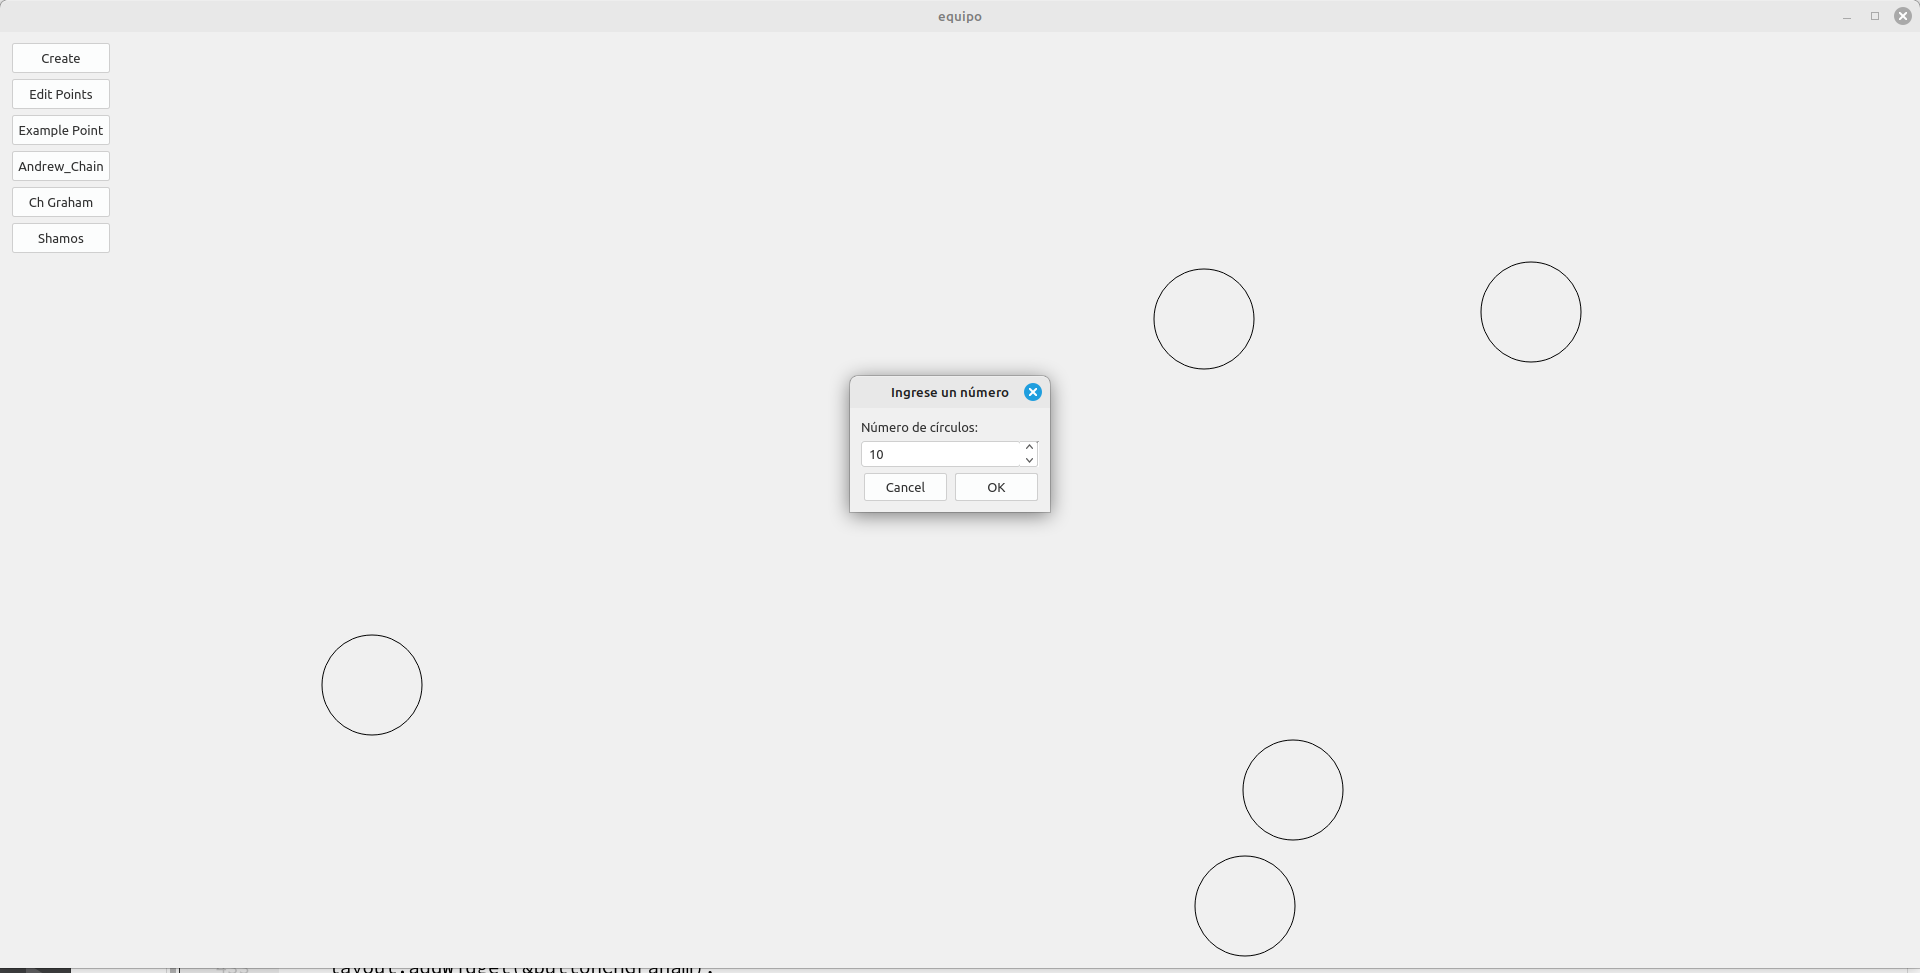
\includegraphics[width=0.8\linewidth]{images/1.png}
    \caption{Interfaz de Edición de Puntos}
    \label{fig:interfaz_edicion_puntos}
    \end{figure}
\end{itemize}


\item \textbf{Interfaz de Inicio del Programa:}
La Figura \ref{fig:interfaz_edicion_puntos} muestra la interfaz de edición de puntos del programa. Al presionar el botón "Edit Points", se abre una ventana emergente que permite al usuario realizar modificaciones específicas en los puntos generados previamente. Esta ventana presenta las siguientes características:

\begin{itemize}
    \item Al hacer clic en cualquier posición dentro de la ventana emergente, se crea un nuevo círculo en esa ubicación, lo que proporciona al usuario la capacidad de añadir puntos adicionales de manera intuitiva y precisa. La ventana de edición incluye tres botones adicionales para mejorar la experiencia del usuario:
    \begin{itemize}
        \item \textbf{Cancelar:} Este botón permite al usuario salir de la ventana emergente sin guardar los cambios realizados, brindando una opción para abortar la operación actual si es necesario.
        \item \textbf{Borrar Dibujo:} Al seleccionar este botón, se borran todos los círculos dibujados en la ventana de edición, lo que ofrece una manera rápida y conveniente de eliminar los puntos existentes y comenzar de nuevo si es necesario.
        \item \textbf{Done:} Al hacer clic en este botón, se confirman y guardan los cambios realizados en la ventana de edición de puntos, permitiendo al usuario finalizar el proceso de edición y regresar a la interfaz principal del programa con los ajustes actualizados.
    \end{itemize}
\end{itemize}

\begin{figure}[h]
    \centering
    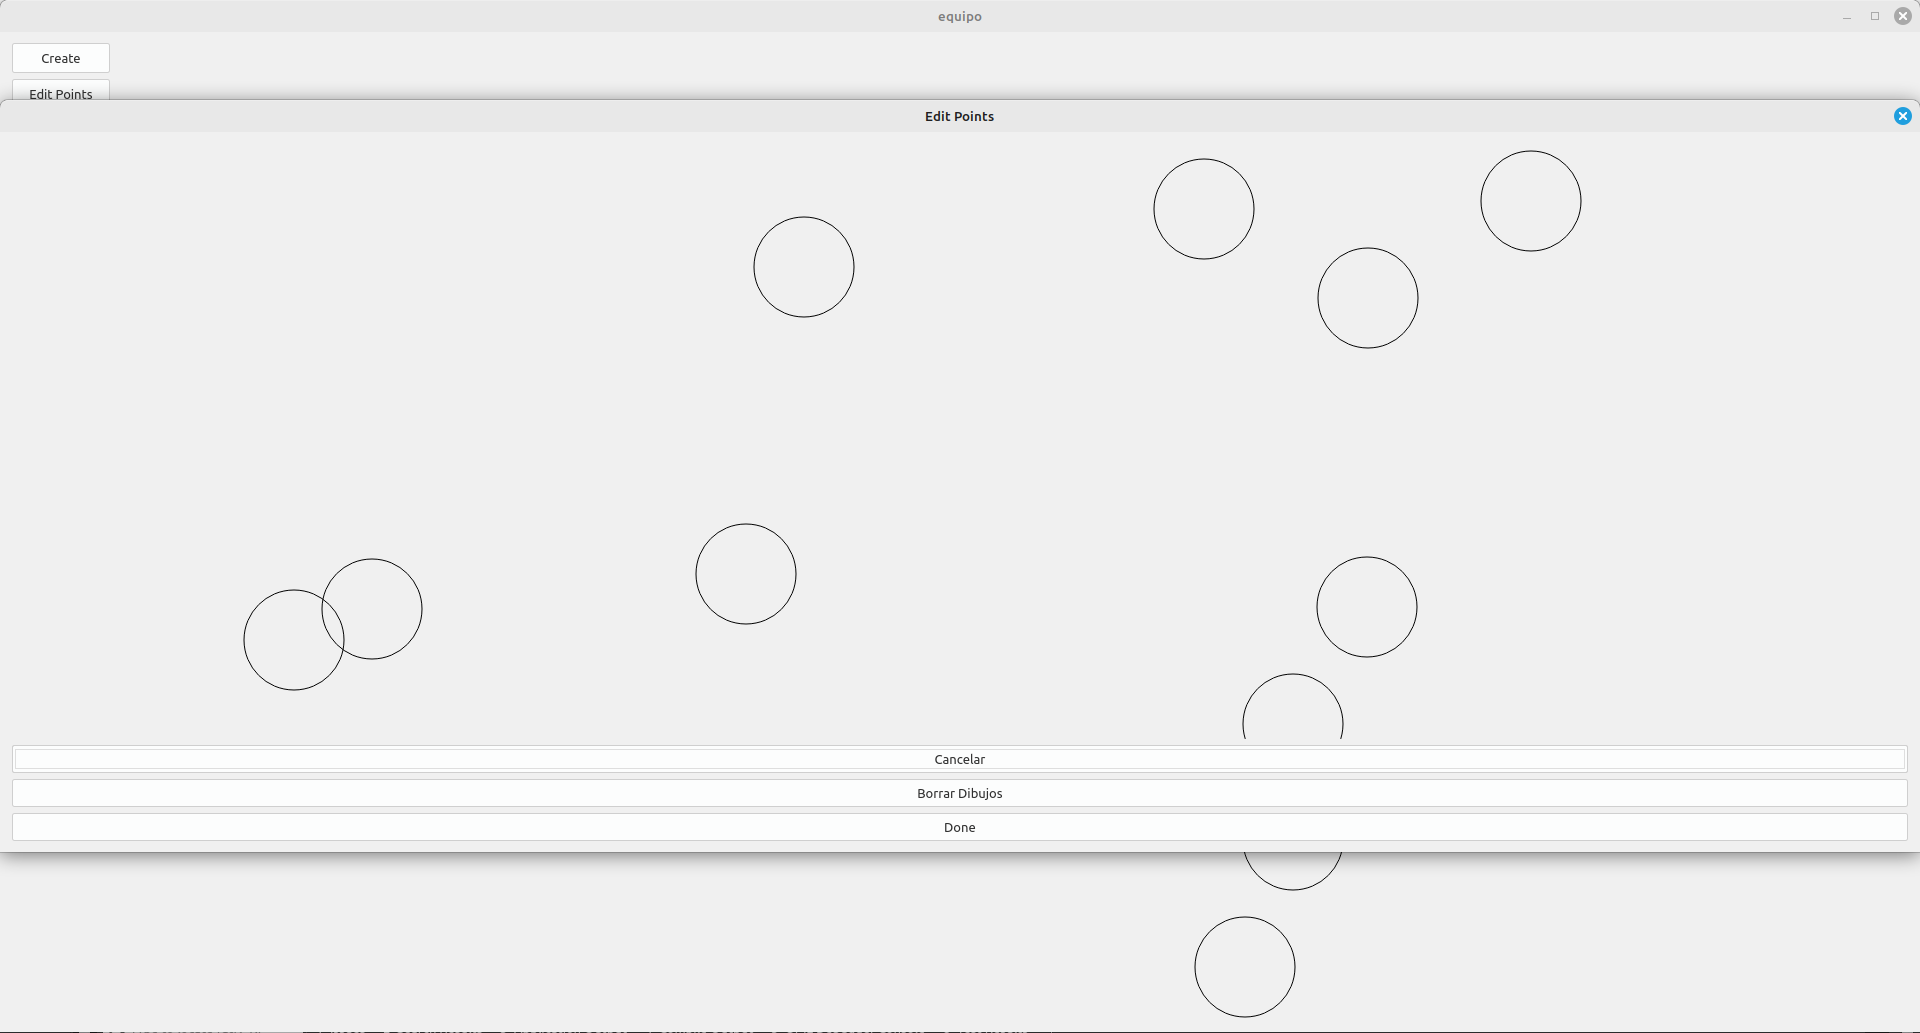
\includegraphics[width=0.8\linewidth]{images/3.png}
    \caption{Interfaz de Edición de Puntos}
    \label{fig:interfaz_edicion_puntos}
    \end{figure}


\item \textbf{Ejemplos de Figuras Generadas:}
La Figura \ref{fig:ejemplos_figuras_generadas} muestra cuatro ejemplos representativos de figuras geométricas generadas a partir de círculos. Estos ejemplos ilustran las siguientes figuras:

\begin{itemize}
    \item \textbf{Cuadrado (Square):} Se muestra un ejemplo de un cuadrado generado mediante la disposición estratégica de varios círculos, demostrando cómo la combinación adecuada de formas básicas puede crear figuras más complejas y reconocibles.
    \item \textbf{Pentágono (Pentagon):} En este ejemplo, se presenta un pentágono formado por la intersección y superposición de múltiples círculos, ilustrando cómo esta técnica puede emplearse para construir polígonos regulares de varios lados.
    \item \textbf{Creciente (Crescent):} Se exhibe un ejemplo de una creciente o luna creciente, modelada mediante la disposición cuidadosa de círculos para simular la curvatura característica de este tipo de figura, mostrando así la versatilidad del enfoque utilizado.
    \item \textbf{Círculo (Circle):} Por último, se incluye un ejemplo simple de un círculo formado por la superposición de varios círculos concéntricos, destacando cómo la técnica puede utilizarse para representar formas básicas con precisión y detalle.
\end{itemize}

Estos ejemplos proporcionan una visualización clara y práctica de las capacidades del programa al generar figuras complejas a partir de la combinación y manipulación de elementos simples, demostrando así su utilidad y versatilidad en la creación de diseños geométricos variados.

\begin{figure}[h]
    \centering
    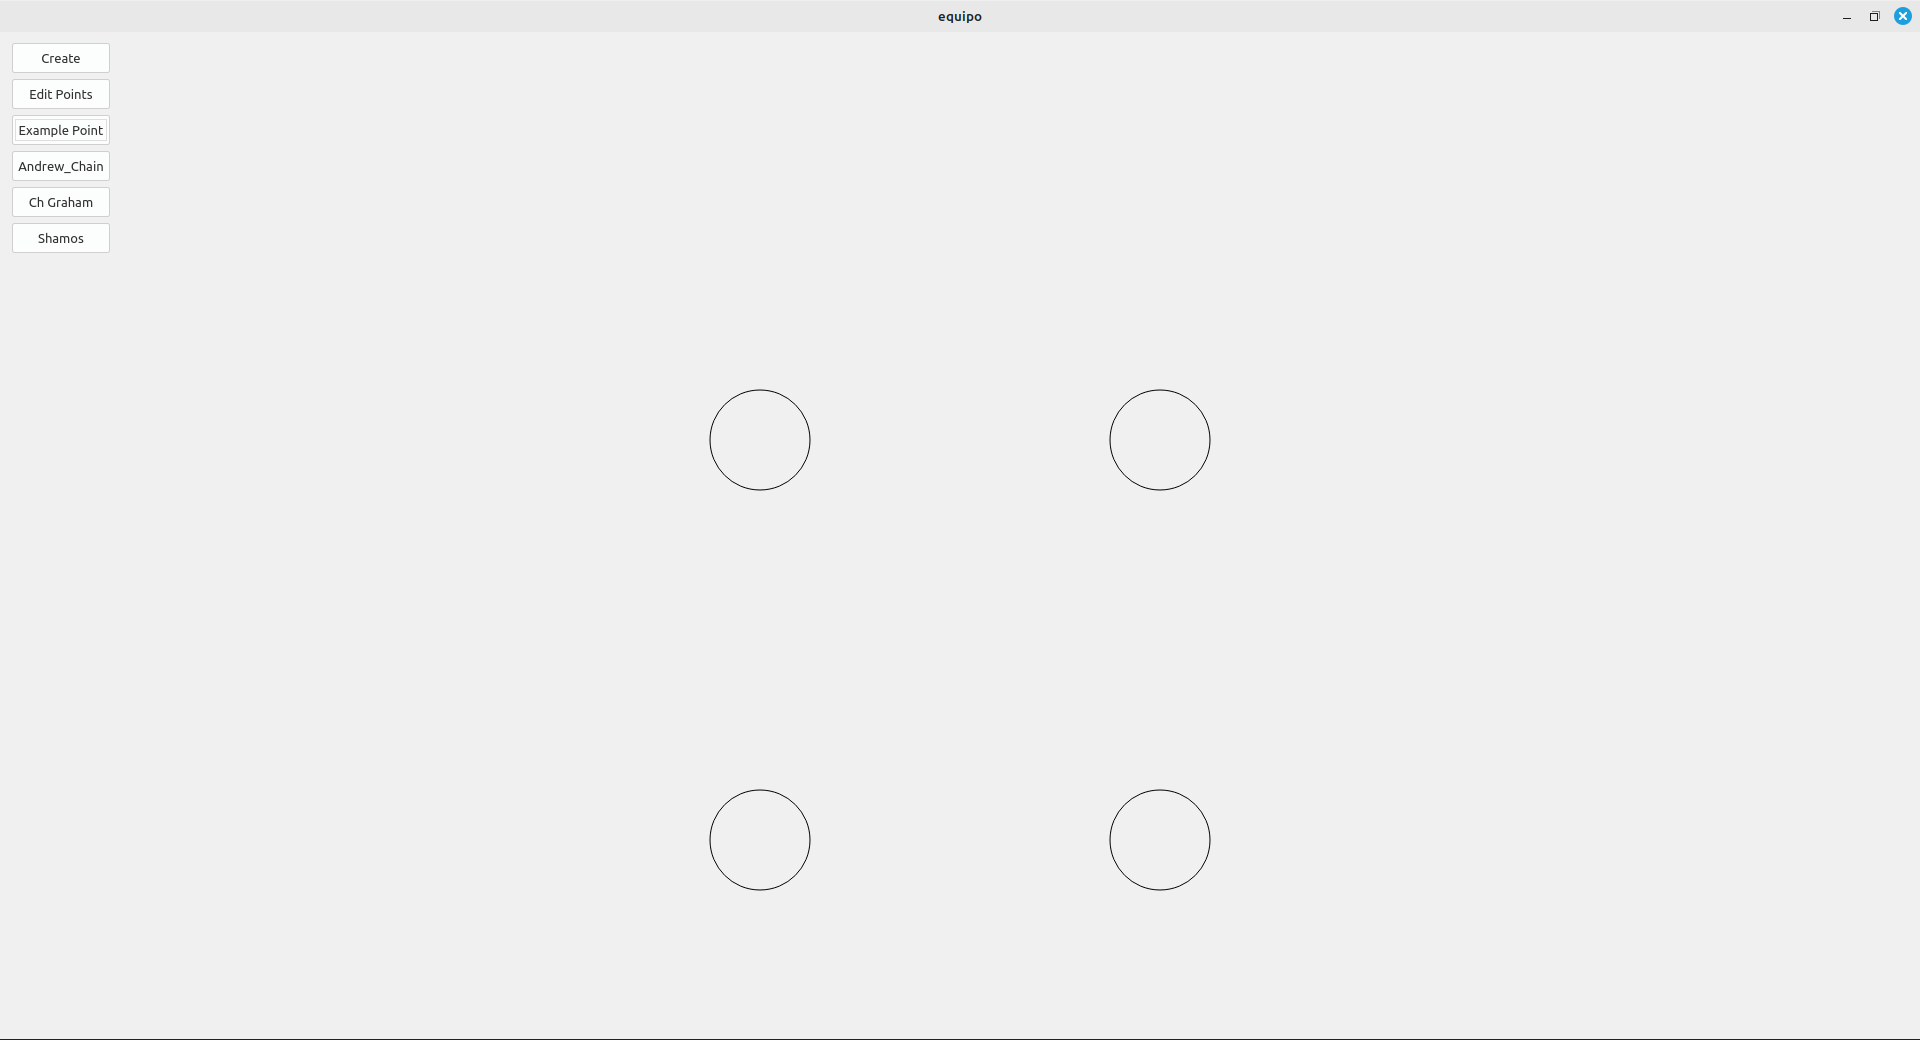
\includegraphics[width=0.8\linewidth]{images/4.png}
    \caption{Ejemplo de Figura Generada (Square)}
    \label{fig:ejemplos_figuras_generadas}
\end{figure}

\item \textbf{Funciones Aplicadas a los Puntos:}
La Figura \ref{fig:funciones_aplicadas} ilustra cómo las funciones Andrew Chain \ref{fig:funcion_an} , Ch Graham \ref{fig:funcion_ch} o Shamos \ref{fig:funcion_sh}  del programa se aplican a los puntos presentes en la pantalla en ese momento. Estos puntos pueden ser generados de tres maneras diferentes:

\begin{itemize}

\begin{figure}[h]
    \centering
    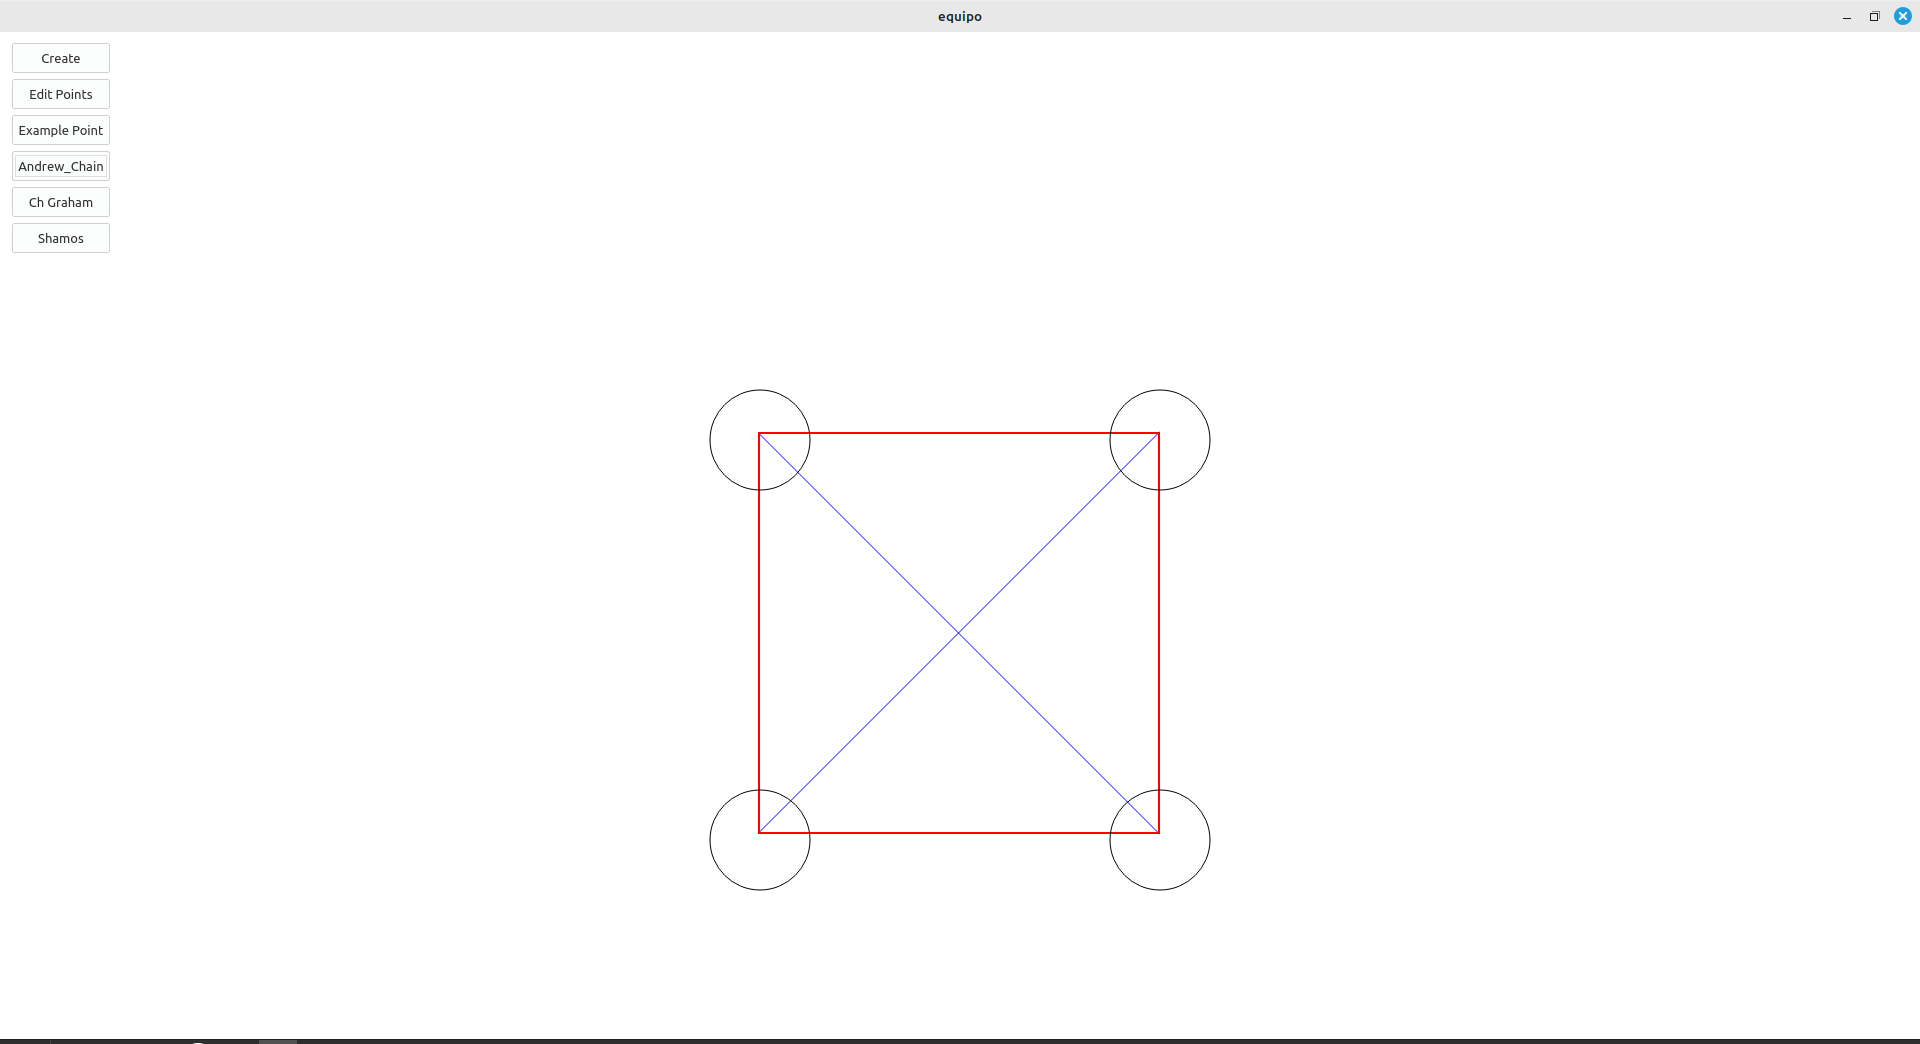
\includegraphics[width=0.8\linewidth]{images/5.png}
    \caption{Funciones Aplicadas a los Puntos}
    \label{fig:funciones_aplicadas}
\end{figure}

    \item \textbf{Ejemplos Predefinidos:} Los puntos pueden ser ejemplos predefinidos proporcionados por el programa, que representan diversas figuras geométricas como cuadrados, pentágonos, crecientes, entre otros.
    \item \textbf{Generados Aleatoriamente:} También es posible que los puntos sean generados aleatoriamente por el programa, lo que permite una variedad de formas y distribuciones para ser procesadas por las funciones seleccionadas.
    \item \textbf{Modificados por el Usuario:} Los puntos pueden ser creados o modificados por el usuario mediante la función de edición de puntos, lo que brinda flexibilidad para personalizar y ajustar las figuras según las necesidades específicas.
\end{itemize}


Al aplicar una de las funciones mencionadas a los puntos presentes en la pantalla, se ejecuta un algoritmo específico diseñado para realizar una tarea particular, como el cálculo de la envolvente convexa (Andrew Chain), la búsqueda del punto más bajo y la ordenación angular (Ch Graham), o la búsqueda de pares de puntos más cercanos (Shamos). El resultado de estas operaciones se visualiza en la pantalla, proporcionando al usuario una representación clara y comprensible de los resultados de la función aplicada a los puntos seleccionados. Esta capacidad del programa permite explorar y analizar de manera interactiva diversas estructuras geométricas y relaciones entre puntos, facilitando la comprensión y el estudio de conceptos clave en geometría computacional.

\begin{figure}[h]
    \centering
    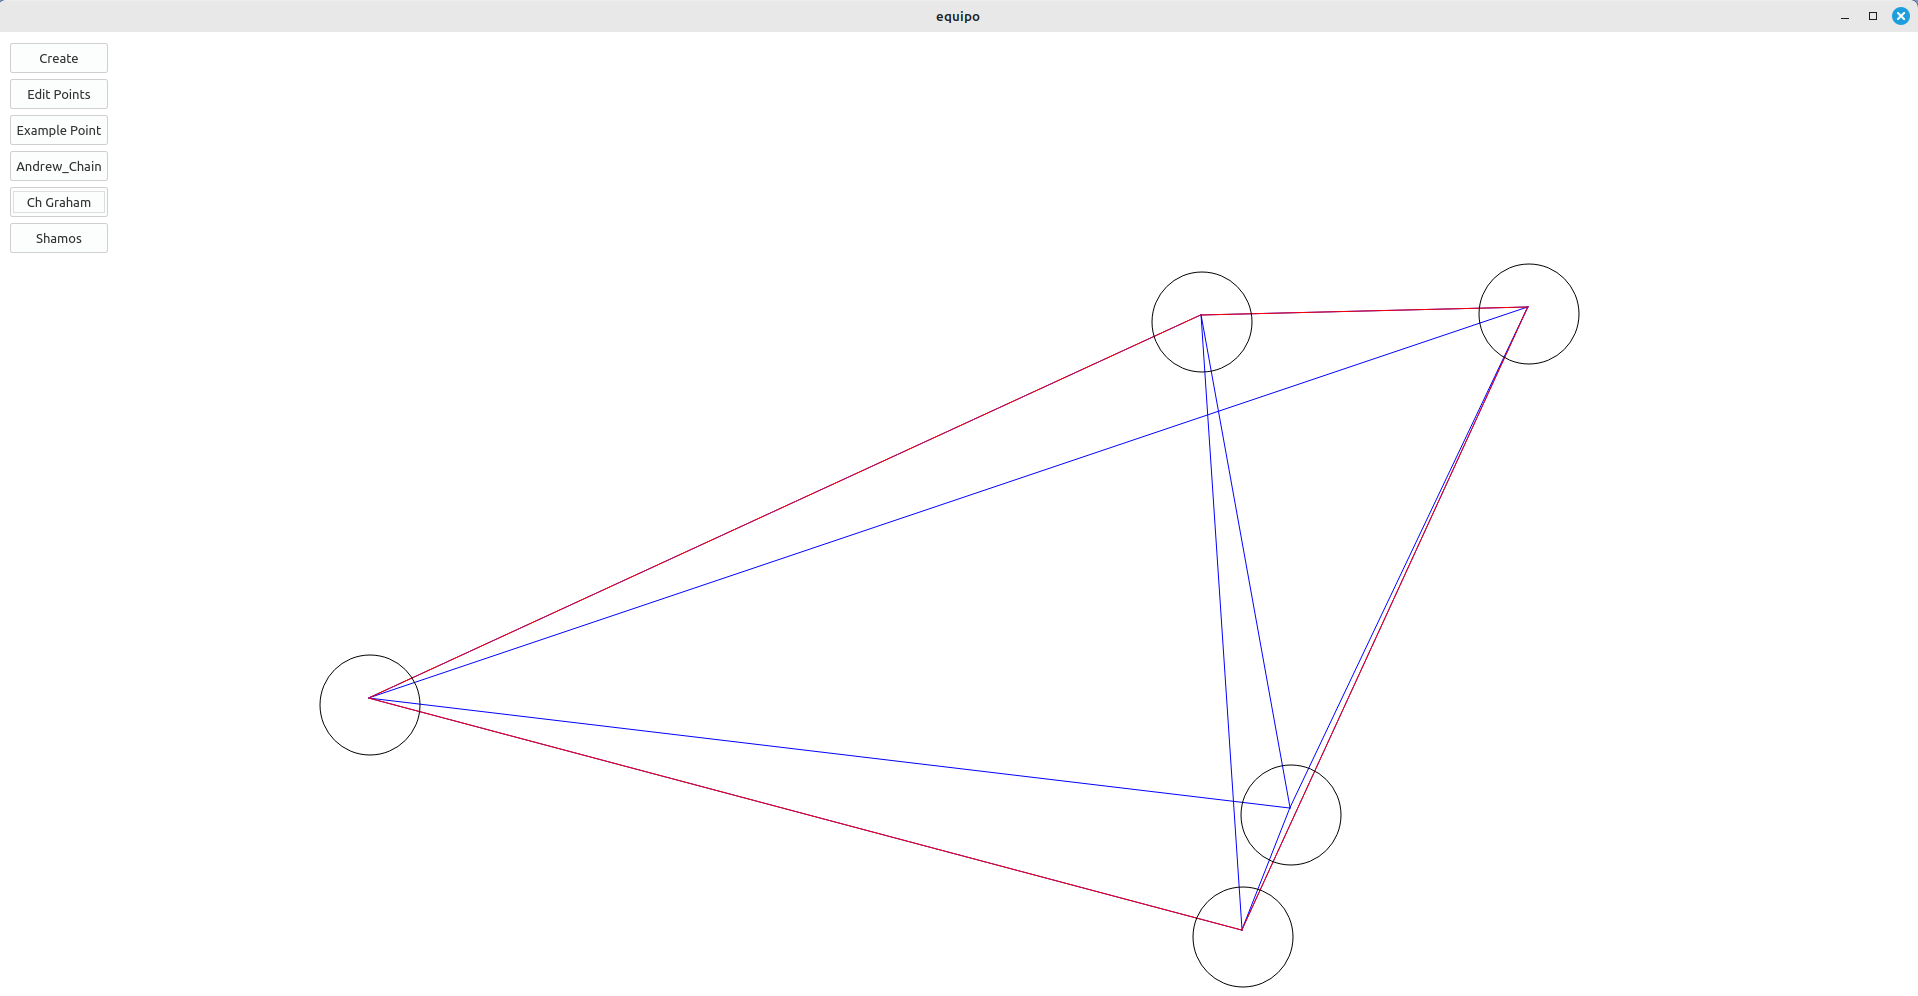
\includegraphics[width=0.8\linewidth]{images/6.png}
    \caption{Funcion de Ch Graham}
    \label{fig:funcion_ch}
\end{figure}

\begin{figure}[h]
    \centering
    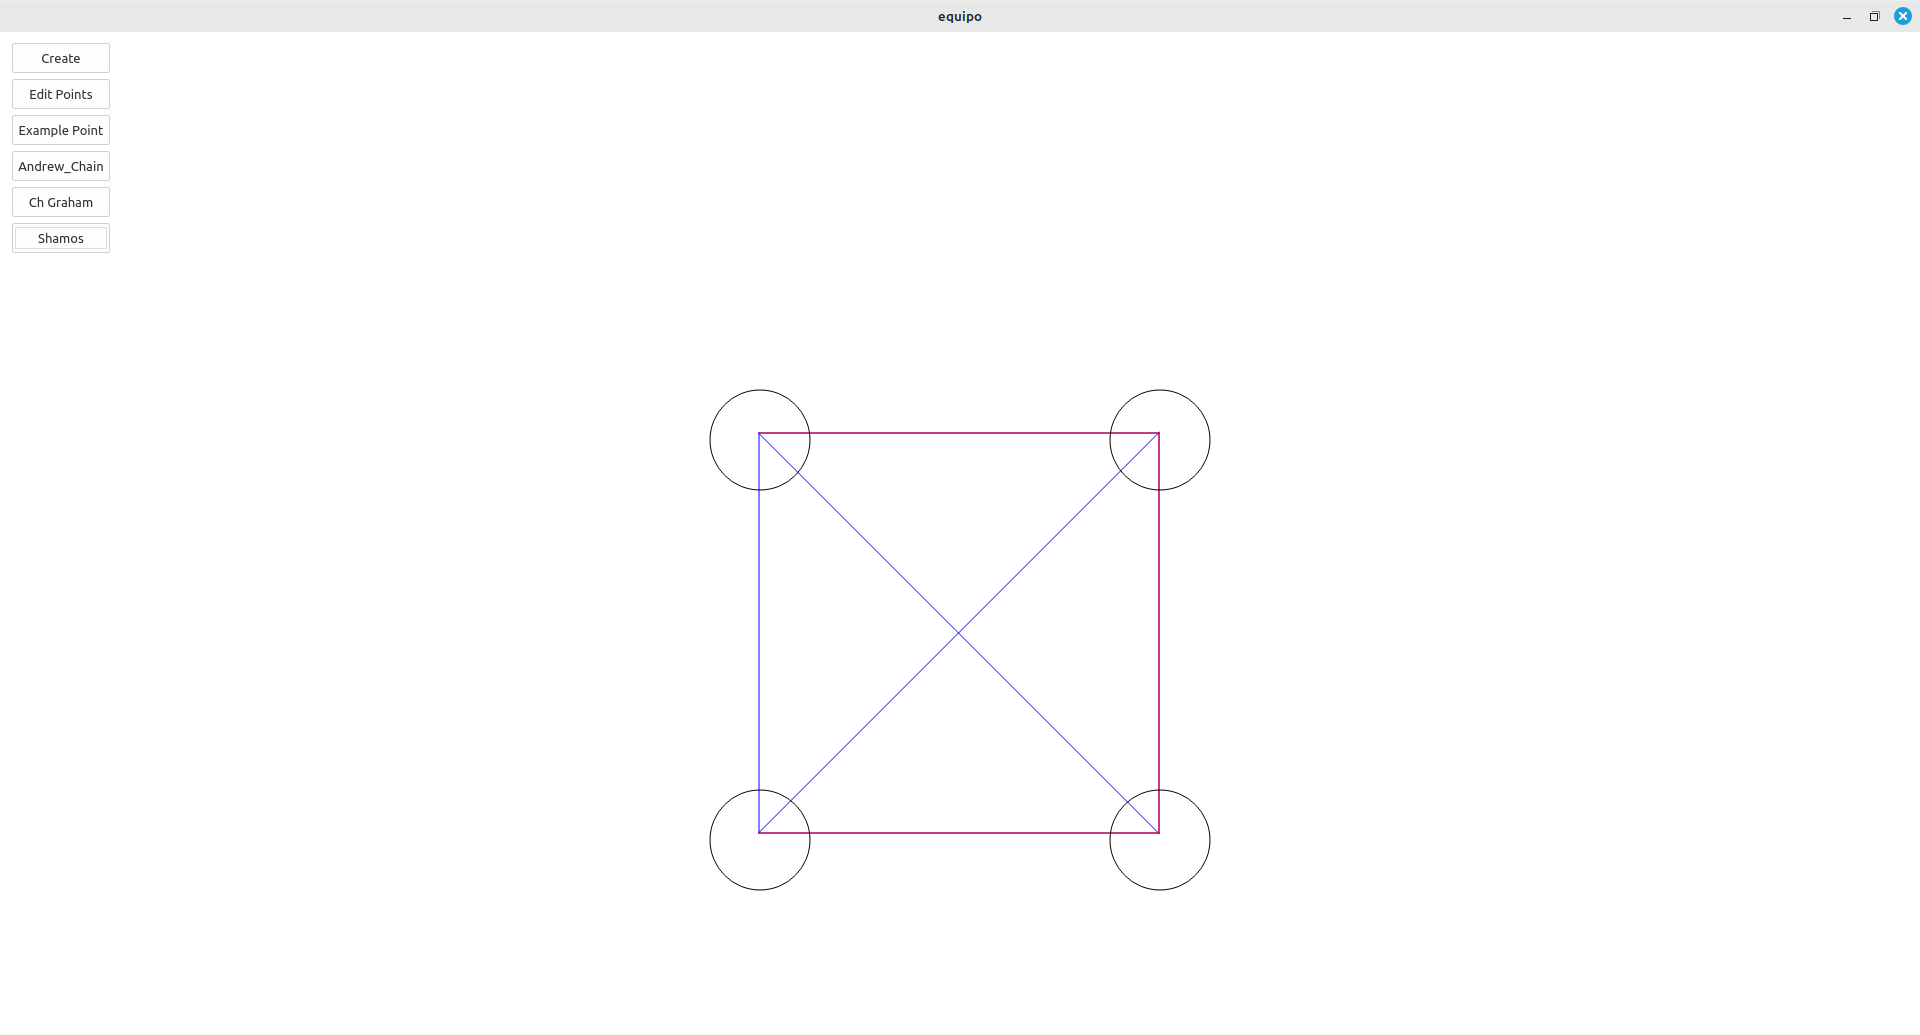
\includegraphics[width=0.8\linewidth]{images/7.png}
    \caption{Funcion de Shamos}
    \label{fig:funcion_sh}
\end{figure}

\begin{figure}[h]
    \centering
    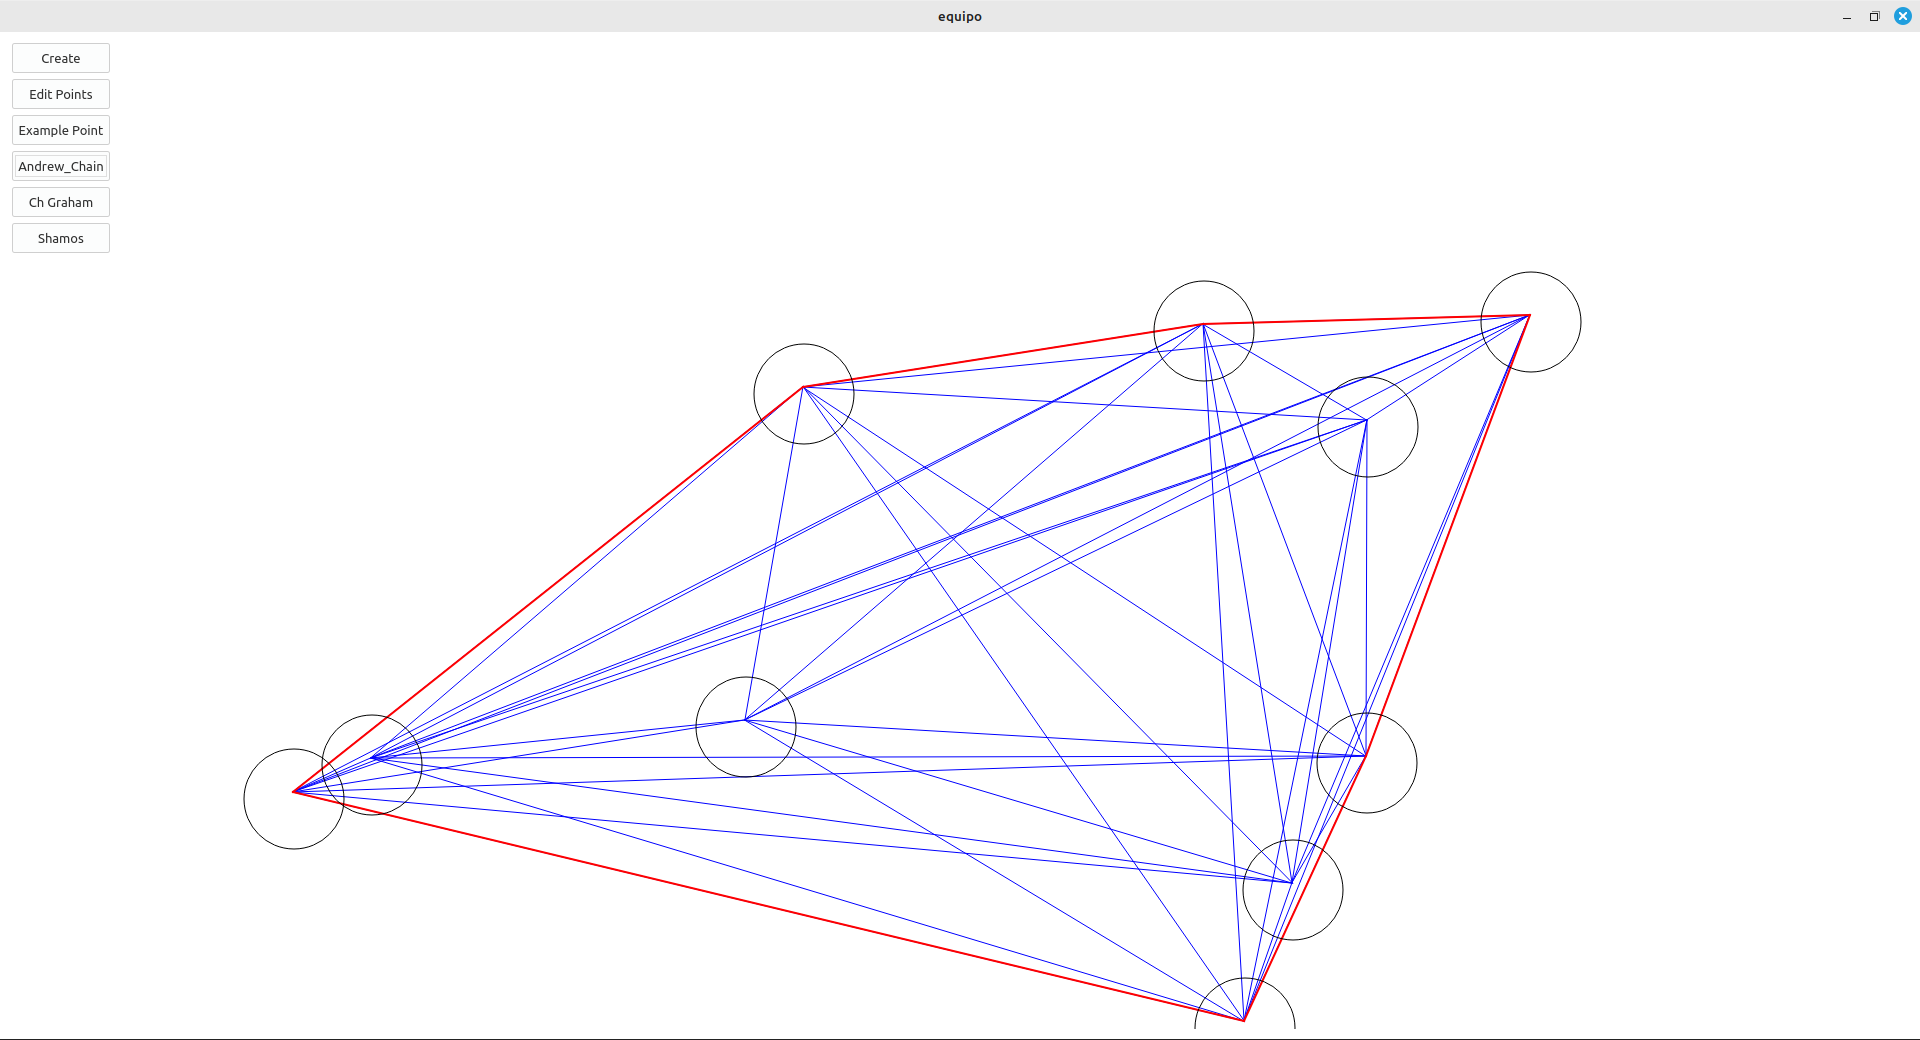
\includegraphics[width=0.8\linewidth]{images/8.png}
    \caption{Funcion de Andrew Chain}
    \label{fig:funcion_an}
\end{figure}

\end{enumerate}


\section{Conclusión}

En conclusión, este proyecto ha logrado con éxito los objetivos establecidos al desarrollar una aplicación en C++ utilizando la biblioteca Qt para resolver el problema de la envolvente convexa. A través de la investigación exhaustiva, el diseño cuidadoso y la implementación efectiva de los algoritmos de Andrew's Monotone Chain, Graham Scan y Shamos, se ha creado una herramienta interactiva y amigable para el usuario.

La aplicación resulta ofrecer una interfaz intuitiva que permite a los usuarios generar conjuntos de puntos, editarlos según sea necesario y aplicar dichos algoritmos para encontrar la envolvente convexa. Los algoritmos implementados funcionan de manera eficiente y producen resultados precisos incluso para conjuntos de puntos grandes.

Por última instancia, este proyecto contribuyó significativamente tanto al crecimiento personal como en equipo, ya que a través del trabajo en equipo se llevó la paciencia, la tranquilidad, la responsabilidad, el esfuerzo y la productividad. También aportando conocimiento teórico y práctico, logrando tener un impacto significativo en diversas áreas, como la geometría computacional, la visión por computadora y el procesamiento de imágenes. Este proyecto proporciona una base sólida para abordar desafíos más avanzados y complejos en futuros trabajos y colaboraciones.


\addcontentsline{toc}{section}{Referencias} 
\printbibliography

\clearpage
\begin{figure*}
\section{Anexos}
    \centering
    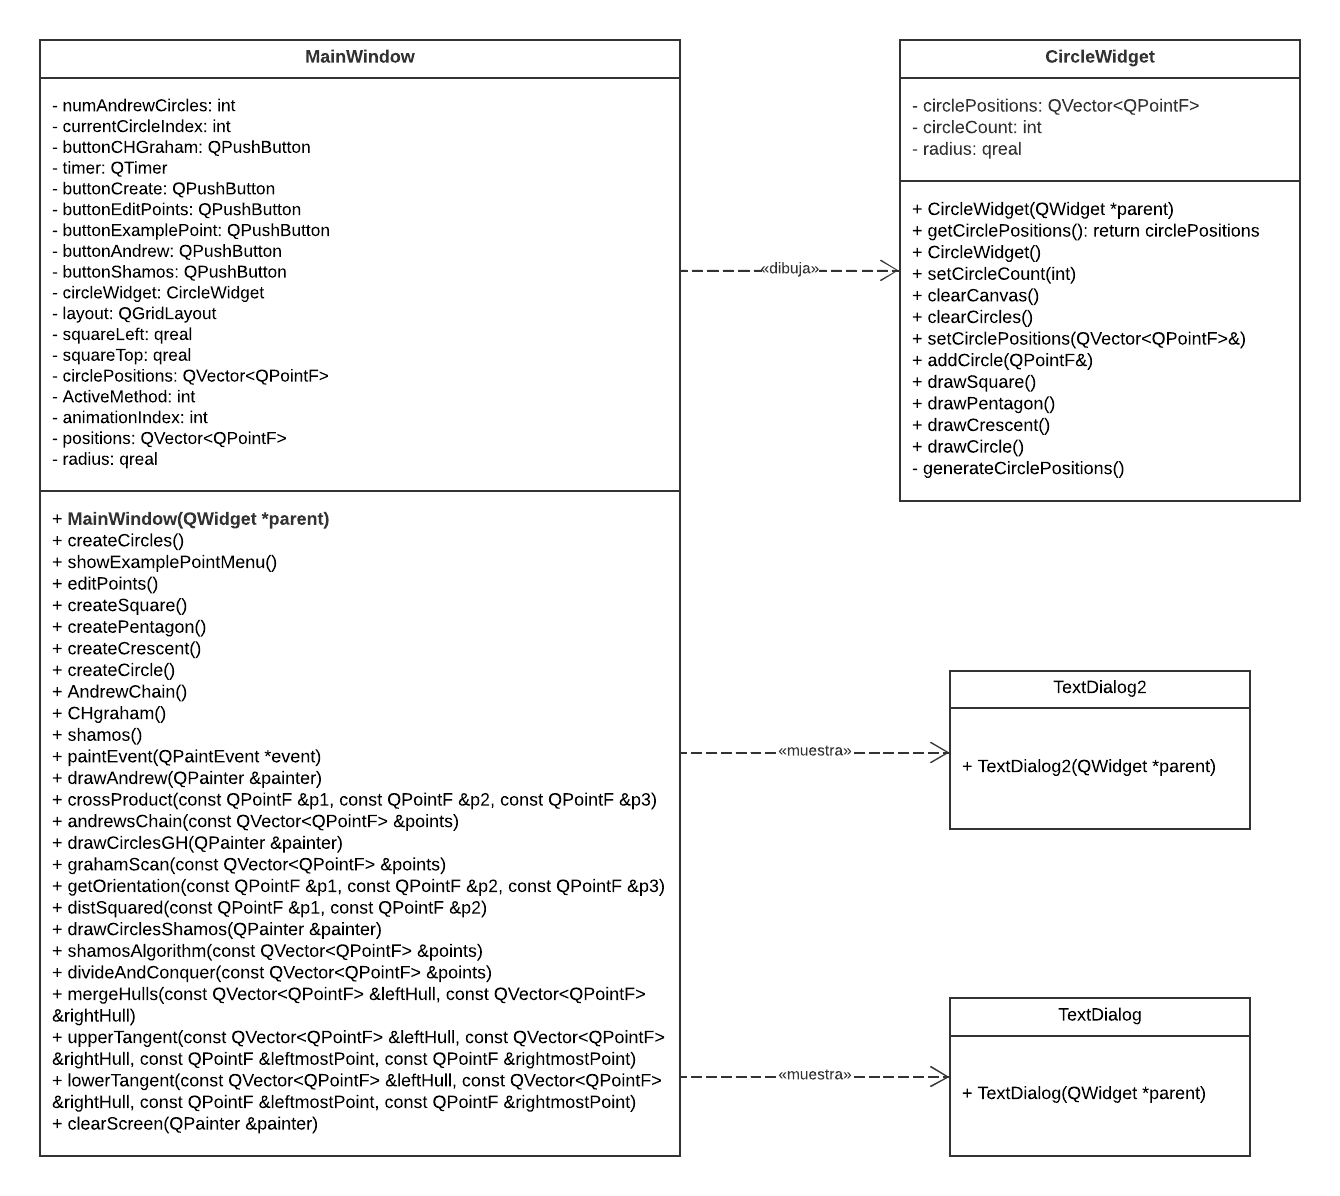
\includegraphics[width=\RelacionFiguradoscolumnas \linewidth]{images/Diagrama de clases.png}
    \caption{Diagrama de clases.}
    \label{fig:DiagramadeClases}
\end{figure*}

\end{document}













